\section{Programming Assignment 3}

\subsection{火焰杯试炼问题}

问题定义为
\begin{itemize}
    \item 动作集合: 上, 下, 左, 右
    \item 状态转移概率: 对于任意非中点格子以及其相邻格子, 若方向匹配, 则有状态转移概率是$1$. 对于终点状态, 转移到初始状态的概率为$1$.
    \item 回报函数: 普通格子的回报为$0$, 陷阱的回报为$-1$, 奖杯的回报为$1$.
\end{itemize}

\subsection{Q-Learning实现}

\lstinputlisting[
    style = Python,
    caption = {\bf update},
    label = {code:rl-update},
    firstline = 268,
    lastline = 293
]{../../homework-programming/pa3/code/maze_env.py}

主要的代码如代码块\ref{code:rl-update}所示, 分为Decision-Making和Learning阶段; 在前一阶段, \\\verb|policy()|函数通过已经记录的Q-Table进行决策, 对于以前没见过的状态, 将所有可能的action的价值初始化为0; 决策时, 有$1-\varepsilon$的概率选择一个价值最高的行动, 对于相同价值的行动则随机选择, 有$\varepsilon$的概率完全随机地选择行动. 在学习阶段, 根据Q-Learning的更新公式更新各个行动的价值.

Q-Table的类型定义为\verb|Dict[State, List[Tuple[Action, float]]]|, 表示某一状态下所有可能的行动以及其对应价值的集合. 设置$\alpha=0.2, \gamma=0.01, \varepsilon=0.01$, 训练智能体, 得到两种情形下的路径长度随探索次数的变化如图\ref{fig:len}.

\begin{figure*}[htbp]
    \centering
    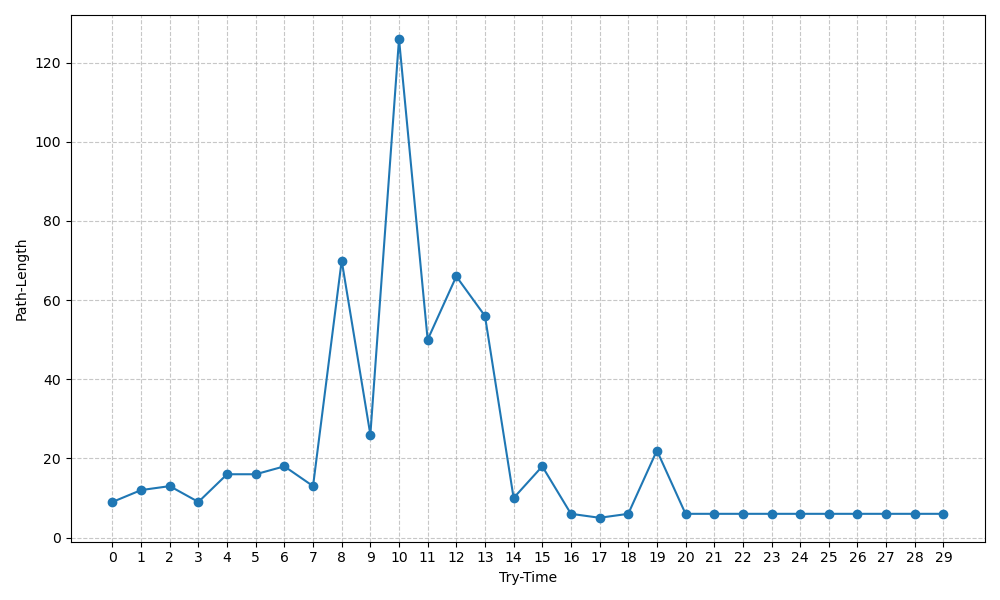
\includegraphics[width=0.6\textwidth]{images/path_len.png}
    \caption{路径长度随探索次数的变化图}\label{fig:len}
\end{figure*}

从图可见智能体一开始的路径长度较短, 说明一直在掉入初始位置附近的陷阱; 之后的路径长度上升, 说明智能体有机会能够探索更远的地方, 但需要花费大量行动去学习; 最后随着偶然几次得到正奖励, 路径长度慢慢降低, 最终收敛到能够稳定到达终点路径. 但由于路径选择存在随机性, 智能体并不一定收敛到最佳路径.

\subsection{Two-Step Q-Learning}

更新公式应当如下: \begin{equation*}
    Q(S_t,A_t) \leftarrow Q(S_t,A_t) + \alpha \left[
        R_{t+1} + \gamma R_{t+2} + \gamma^2 \max_{a\in A} Q(S_{t+2}, a) - Q(S_t,A_t)
    \right]
\end{equation*}

其中$S_t$为$t$时刻的状态, $R_t$为在时间$t$获得的奖励. 更新时机应当是在获得$R_{t+2}$后进行, 即两步之后更新.
